\documentclass[conference]{IEEEtran}
\usepackage{graphicx}
\usepackage{float}  % Needed for the 'H' specifier

% Ensure single spacing
\linespread{1}

\title{\textbf{Pokemon Rank Classifier}}
\author{\textbf{ECS 171 Machine Learning} \\\\Group Leader: Alex D'Souza \\ Group Members: Catherine Chen, Varun Wadhwa, Shane Kim}
\date{\textbf{Github Repository: }https://github.com/AlexanderDsouza/ECS171GroupProject}

\begin{document}
    \maketitle
\chapter{Introduction and background}
Pokemon is one of the most popular franchises in the world, with various console games, mobile apps, and a very passionate trading card collecting community. There are over 8 million daily Pokemon Go players, over 480 million lifetime console game sales, and over 3.7 billion pokemon cards sold in the 2020-2021 fiscal year. The biggest pokemon tournament is the Pokemon World Championship with over 110,000 USD in prize money, so every advantage a player can get is extremely valuable. A big advantage that players can get is being able to categorize pokemon with regards to their strength level. There are a couple of reasons this is advantageous: 

\begin{center}
\textbf{1. Accurately measuring the overall strength of a team}
\end{center}
Tournaments ban certain pokemon that are considered too “strong” so a player’s team will be made up of pokemon from various strength levels. Therefore, to know the overall strength of a player’s roster, knowing the individual strength of each pokemon is crucial. Being able to accurately measure the overall strength of a team also allows a player to know how their roster stacks up against an opposing player’s roster. This allows players to strategically choose pokemon to fill their team as well as determine movesets 

\begin{center}
\textbf{2. Efficient Training}
\end{center}
A Pokemon’s base stats can be improved via a concept known as Effort Values by battling other pokemon. Therefore knowing the strength level of an individual pokemon can allow a player to determine which pokemon need to be trained more.\\

\begin{center}
\textbf{3. Predictions}
\end{center}
Knowing the objective strength level of a pokemon, allows a player to predict what moves their opponent will make against theirs. If a pokemon is “strong” , moves that lower its attack or defense stats may be used. If a pokemon is weak, one shot moves may be preferred.\\ 

\noindent The current issue around categorizing pokemon is that there is no single statistic that determines if a pokemon is strong. For example, one pokemon may have strong attack statistics and one pokemon may have strong defense statistics so in order to determine which pokemon is stronger, various statistics must be considered. Even if an individual is able to manually categorize all 1021 pokemon using their own methodology, new pokemon are frequently released, so manually evaluating each pokemon and comparing them to create strength tiers is not feasible. Machine learning poses an elegant solution to this issue, as being able to produce strength level predictions for new pokemon based on previous generation data without manually having to evaluate and categorize new pokemon saves valuable time.

\chapter{Literature Review}
\begin{center}
\textbf{1. Previous Attempts:}
\end{center}
\begin{itemize}
                \item **Breddan** attempted to predict or categorize attributes of Pokemon, investigating relationships between different statistics such as type, HP, attack, defense, special attack, special defense, speed, and total strength.
                \item Explored whether distinct groups of Pokemon could be formed based on these statistics to aid team diversification.
                \item Attempted to predict one statistic of a Pokemon based on others to anticipate new Pokemon's stats using educated guesses.
            \end{itemize}
            
\begin{center}
\textbf{2. Methodology Used:}
\end{center}
\begin{itemize}
                \item Employed k-means classification and Random Forest Regression techniques.
            \end{itemize}
            
\begin{center}
\textbf{3. Findings:}
\end{center}          
            \begin{itemize}
                \item Successfully created 5 distinct groups of Pokemon using k-means classification with speed and HP data.
                \item Predicted total strength using Random Forest Regression with a maximum tree depth of 11, achieving an accuracy of 95%.
            \end{itemize}
            
    \chapter{Dataset Description}
  The dataset used in this project is a CSV file obtained from Kaggle, generated by scraping pokeapi.co through Python. It comprises 1017 rows and 18 columns, featuring the following attributes:

\begin{itemize}
    \item \textbf{Columns:} 
    \begin{itemize}
        \item ID of the Pokemon
        \item Name
        \item Rank (strength level)
        \item Generation
        \item Evolution chain
        \item Primary type
        \item Secondary type
        \item HP
        \item Attack
        \item Defense
        \item Special attack
        \item Special defense
        \item Speed
        \item Total stats
        \item Height
        \item Weight
        \item Abilities
    \end{itemize}
\end{itemize}

For our model, we decided to consider only numerical data as input features, excluding categorical features such as primary type, secondary type, abilities, evolution information, and others. We made this choice because including these categorical features via one-hot encoding would significantly increase the model's complexity and training time.

Our target variable, Rank, serves as a measure of strength and encompasses four categories: legendary, mythical, baby, and ordinary. We identified 'baby' and 'ordinary', as well as 'mythical' and 'legendary', as redundant labels concerning strength levels. Consequently, we categorized all 'baby' Pokemon as 'ordinary', and 'mythical' as 'legendary'.
    \begin{figure}[H]
        \centering
        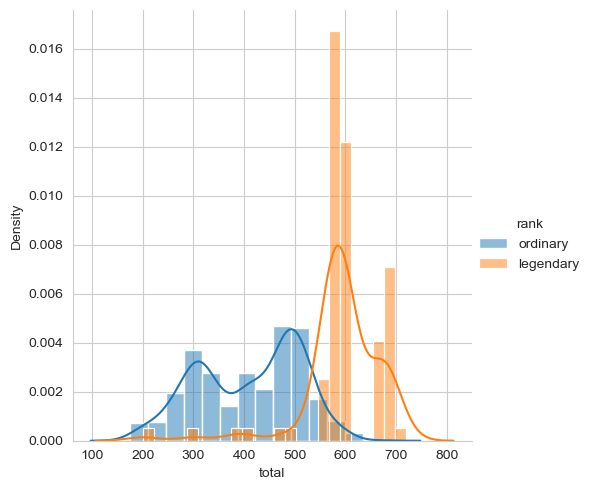
\includegraphics[width=0.8\textwidth]{histplot.png} % Adjust the width as needed
        \caption{Histogram of the Dataset}
        \label{fig:dataset-hist}
    \end{figure}
  This section provides a description of the dataset used in our study. To illustrate the characteristics of the dataset, we include a histogram plot shown in Figure \ref{fig:dataset-hist}. As you can see at around 550 in total stats, legendary Pokemon and ordinary Pokemon make a distinct split. When we saw this, we decided that a linear SVM model would be perfect for our dataset as you can clearly draw a line right in between that mark and it could split the classes pretty accurately. 

    \begin{figure}[H]
        \centering
        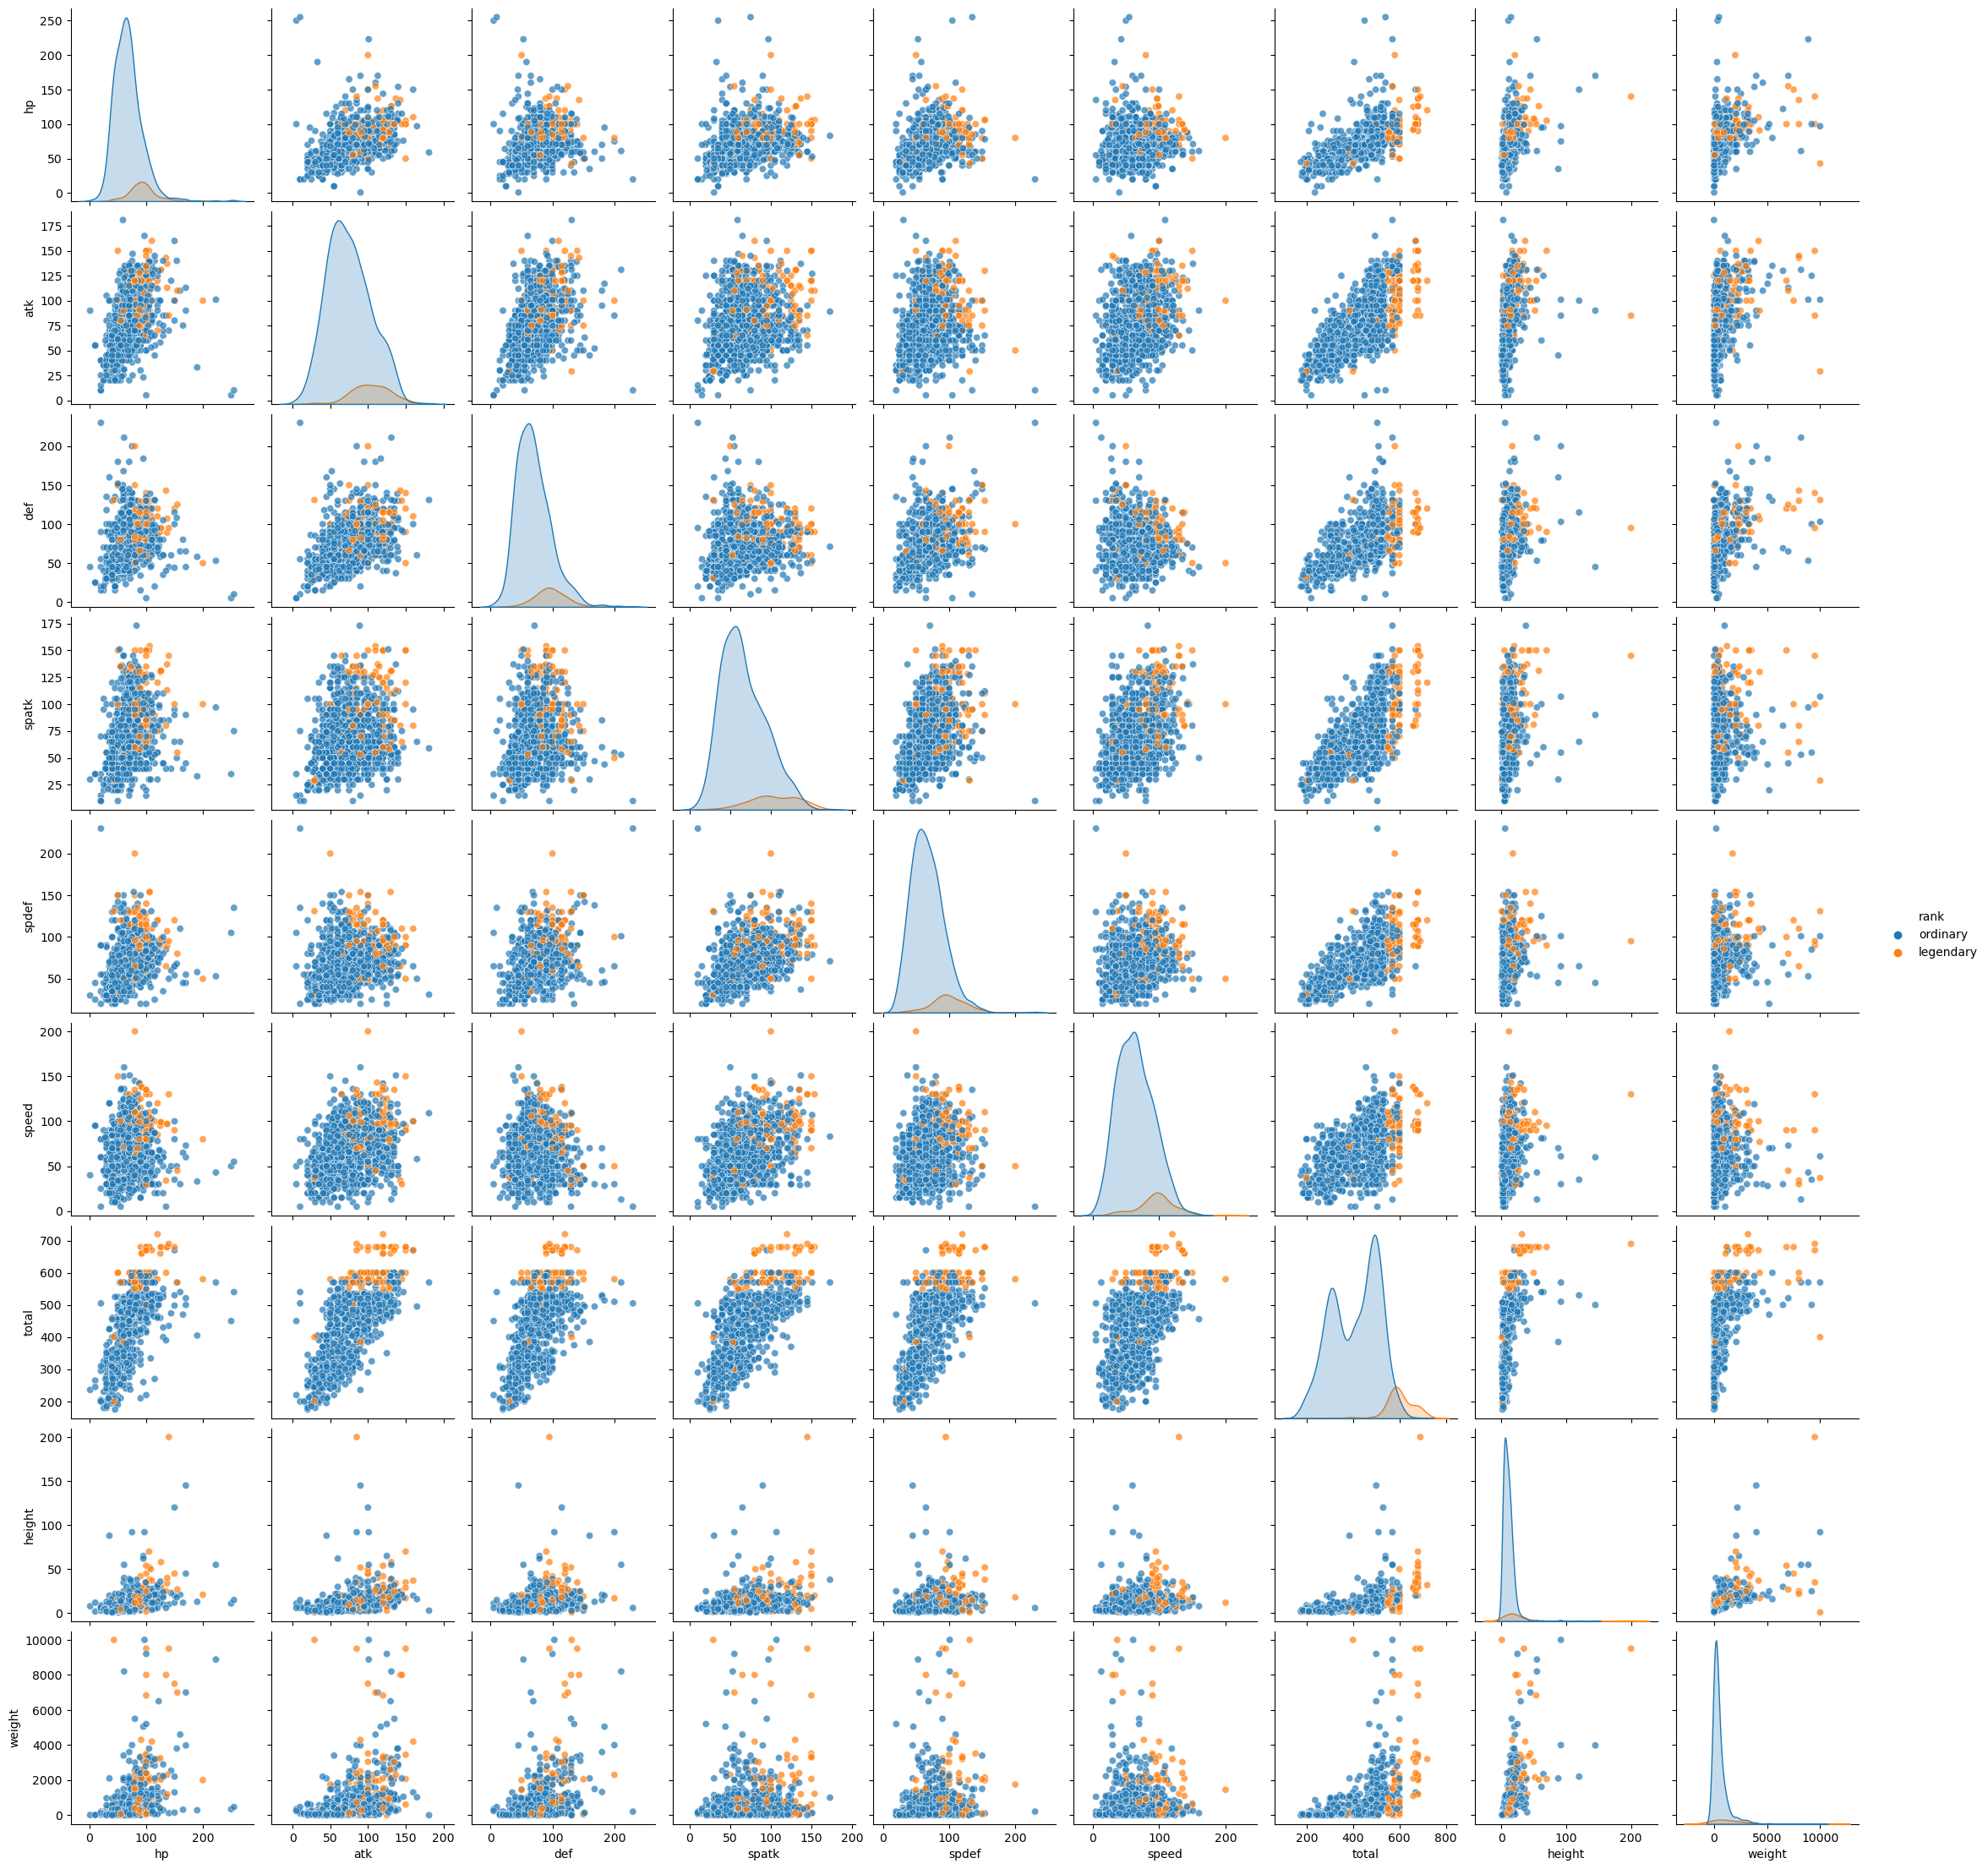
\includegraphics[width=0.8\textwidth]{pairplot.png} % Adjust the width as needed
        \caption{Pair Plot of the Dataset}
        \label{fig:dataset-pairplot}
    \end{figure}
In the pairplot we can also see that in the total pairplots, we can easily cut the classes and group them with a line. This also led us to believe SVM would be extremely good. 

	\chapter{Proposed Methodology}
\section{Model selection}
For our Pokemon rank classifier, we opted to utilize Logistic Regression and Support Vector Machine (SVM) models due to their distinct advantages and capabilities in handling this classification task.

\subsubsection{Logistic Regression}
\textbf{Pros:}
\begin{itemize}
    \item Well-suited for binary classification problems like ours.
    \item Offers probabilistic interpretation of results.
    \item Generally less prone to overfitting.
\end{itemize}

\textbf{Cons:}
\begin{itemize}
    \item Assumes linear relationship between features and the log-odds of the outcome.
    \item May not perform optimally with non-linear data distributions.
\end{itemize}

\subsubsection{Support Vector Machine (SVM)}
\textbf{Pros:}
\begin{itemize}
    \item Effective in high-dimensional spaces.
    \item Versatile due to different kernel functions.
    \item Robust against overfitting in high-dimensional spaces.
\end{itemize}

\textbf{Cons:}
\begin{itemize}
    \item Computationally intensive with larger datasets.
    \item Choice of kernel and parameters crucial for performance.
\end{itemize}

\subsection{User Prediction Interface}

Our classifier allows users to predict whether a chosen Pokemon is legendary or not. Initially, we considered enabling users to specify the Effort Values (EVs) of the Pokemon. However, for simplicity and consistency with our test data, users can select a Pokemon, and our system will randomly distribute their EVs within allowable constraints.

\subsection{Data Augmentation}

To enhance our dataset and balance class representation, we augmented the dataset by generating additional data points. We increased the representation of 'legendary' Pokemon to ensure robustness in the training phase.

\subsection{Model Training and Evaluation}

\textbf{Data Preprocessing:} We preprocessed the data, removing unnecessary features and ensuring numerical consistency.

\textbf{Model Training:} We trained both Logistic Regression and SVM models on the augmented dataset.

\textbf{Model Evaluation:} Using train-test splitting, we evaluated the models' performance and obtained classification reports for each model.

\subsection{Model Persistence}

Upon successful training and evaluation, we persisted the SVM model as 'Pokemon\_Predictor.pkl', enabling the deployment of the trained model for future predictions.
    

    \chapter{Experimental Results}
    \chapter{Conclusion and Discussion}
    \chapter{References}
\end{document}
